\subsection{Funktionsanalyse}

\textit{(pro)} In diesem Kapitel wird der Planting Robot in verschieden Funktionsblöcke zerlegt. Die dadurch definierten Teilfunktionen ermöglichen ein systematisches Maschinendesign. Zu den jeweiligen Funktionsblöcken werden in Kapitel \ref{funktionsbez_var} verschiedene Lösungsvarianten ausgearbeitet. Diese Teilkonzepte werden anschliessend in Kapitel \ref{konzept} zu einem kompletten Maschinendesign zusammengeführt.\newline
Bei der Funktionsanalyse wird zwischen einer Pflicht und einer komplexeren Wunschanforderung unterschieden. Die Wunschanforderung beschreibt zusätzlich zum vollen Funktionsumfang, eine selbstständig Konfiguration des Planting Robots auf verschieden Topfgrössen.


\begin{figure}[H]
	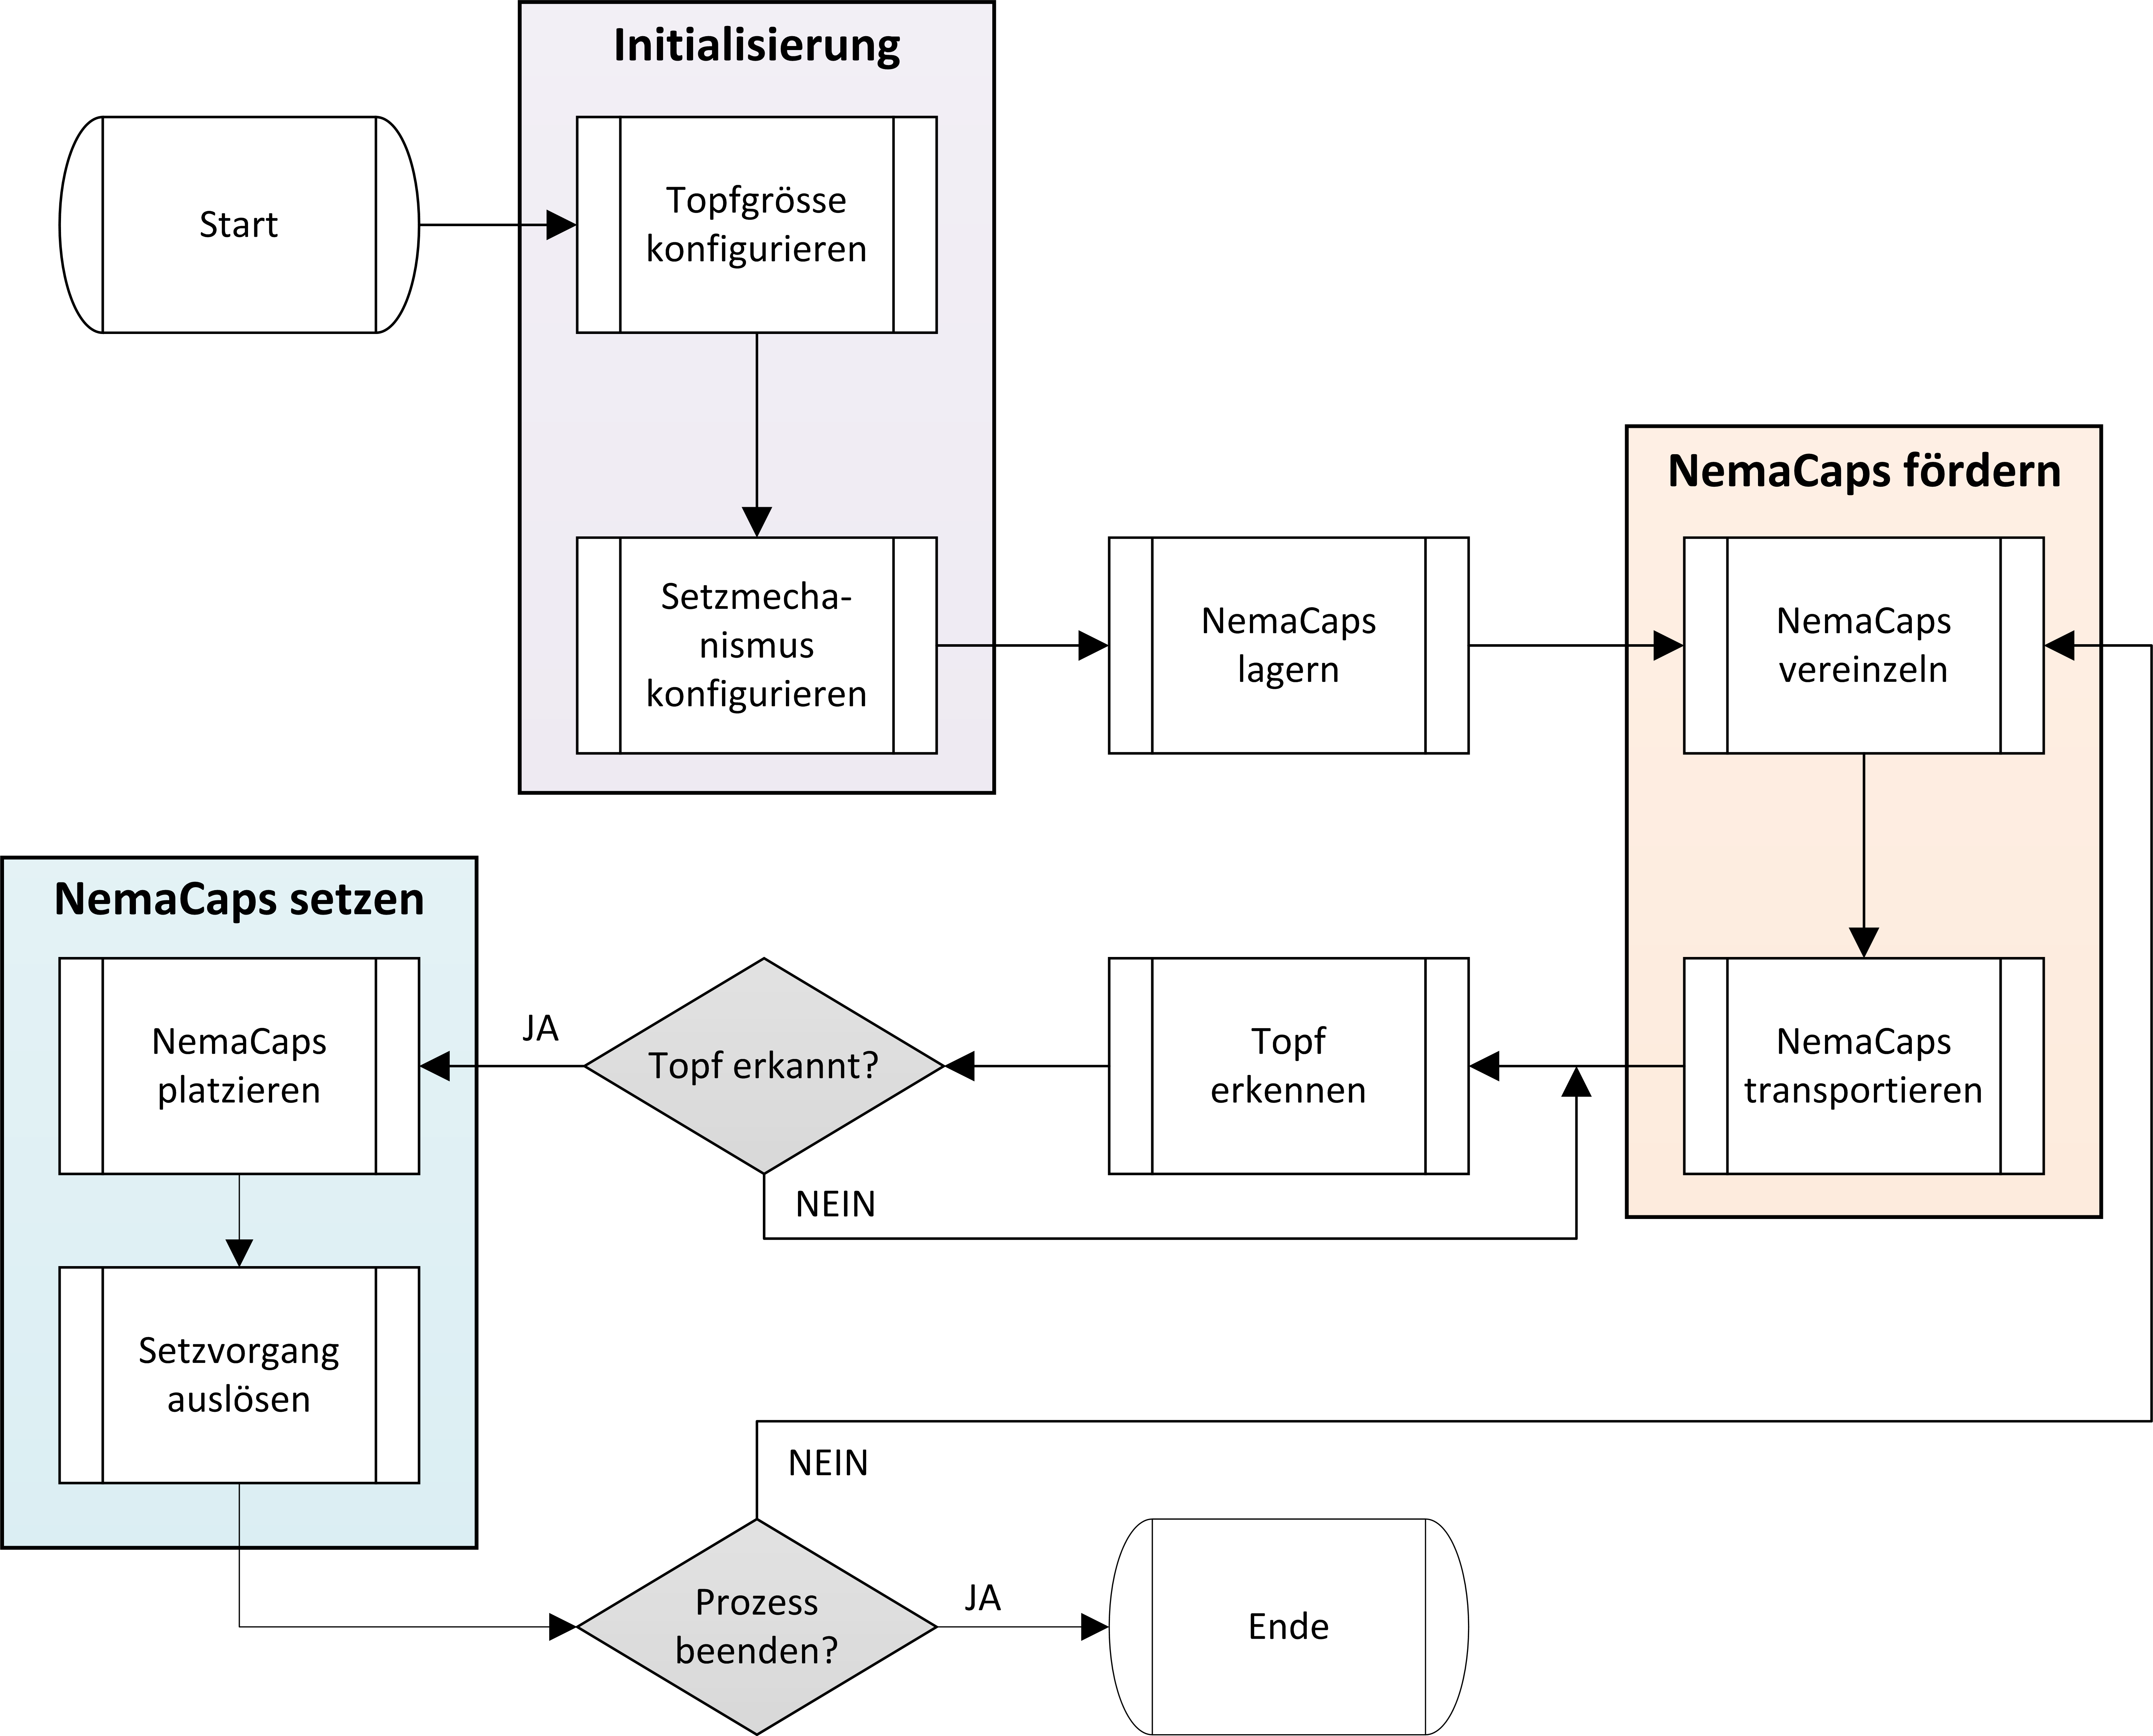
\includegraphics[width=0.8\textwidth]{Illustrationen/4-Entwurf/Funktionsanalyse_Pflicht.png}
	\caption{Funktionsanalyse Pflicht Blockdiagramm}
	\label{fig:FunktPflicht}
\end{figure}

\begin{itemize}
	\item \textbf{Initialisierung:} Die Initialisierung wird durch einen Operator ausgeführt. Diese Teilfunktion ist nur in der Pflichtanforderung vorhanden, da die Maschine im Umfang der Pflichtanforderung die Initialisierung nicht selbstständig durchführt.
	
	\begin{itemize}
		\item \textbf{Topfgrösse konfigurieren:} In diesem Funktionsblock wird an der Maschine über ein HMI die verwendete Topfgrösse eingestellt.

		\item \textbf{Setzmechanismus konfigurieren:} Der Setzmechanismus muss für verschiedene Topfgrössen eingestellt oder ausgetauscht werden.
	\end{itemize}
	
	\item \textbf{NemaCaps lagern:} Das Setzgut (NemaCaps) wird in der Maschine mit einem Bestand von bis zu 10'000 Einheiten gelagert.
	
	\begin{figure}[H]
		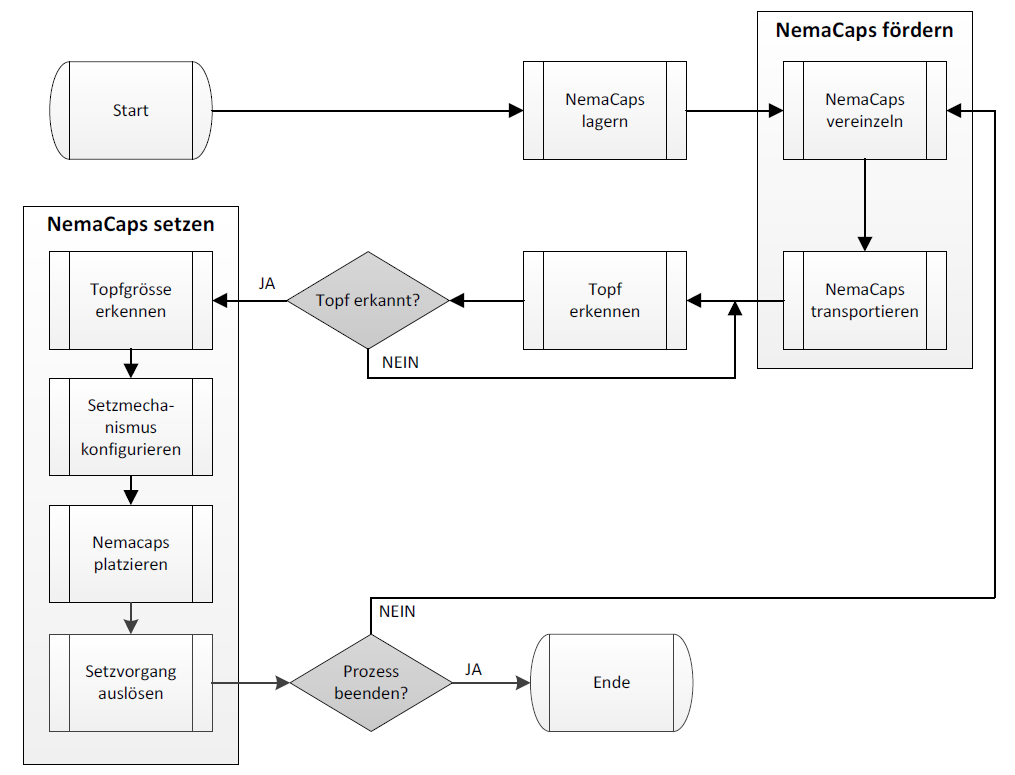
\includegraphics[width=0.8\textwidth]{Illustrationen/4-Entwurf/Funktionsanalyse_Wunsch.png}
		\caption{Funktionsanalyse Wunsch Blockdiagramm}
		\label{fig:FunktWunsch}
	\end{figure}
	
	\item \textbf{NemaCaps fördern:} Diese Teilfunktion behandelt die Verbindung zwischen Lager und Setzmechanismus.
	
	\begin{itemize}
		\item \textbf{NemaCaps vereinzeln:} Um die NemaCaps gezielt und kontrolliert in die Topferde einsetzen zu können, werden diese vor dem Setzen vereinzelt.
		
		\item \textbf{NemaCaps transportieren:} Der Transport zwischen Lager und Setzmechanismus kann vor oder nach der Vereinzelung stattfinden.
	\end{itemize}




	\item \textbf{Topf erkennen:} Diese Teilfunktion übernimmt implizit zwei Aufgaben. Es soll erkannt werden, ob ein Topf für den Setzprozess bereit steht und ob sich dieser in Bewegung ist oder nicht. 
	
	\item \textbf{NemaCaps setzen:} Erst wenn ein Topf bereit steht, wird der Setzprozess eingeleitet. Dieser unterscheidet sich, wie in Abb. \ref{fig:FunktPflicht} und Abb. \ref{fig:FunktWunsch} ersichtlich, zwischen Pflicht und Wunschanforderung anhand des Funktionsumfangs.
	
	\begin{itemize}
		\item \textbf{Topfgrösse erkennen:} Durch Sensorik soll die Topfgrösse jedes Topfes vermessen werden.
		
		\item \textbf{Setzmechanismus konfigurieren:} Anhand der gewonnen Daten zur Topfgrösse, soll die Maschine den Setzmechanismus selbstständig adaptieren.
		
		\item \textbf{Nemacaps platzieren:} Es folgt der eigentliche Setzprozess, in welchem die Nemacaps in einer definierten Anordnung in Position gebracht werden.
		
		\item \textbf{Setzvorgang auslösen:} Die Nemacaps welche vorher in Position gebracht wurden, werden nun in diesem Schritt vom Setzmechanismus in die Erde befördert.
	\end{itemize}
	
\end{itemize}
